\scanpage{82}

§. \uline{Convexity inequalities and remarkable degrees of operators, compact}

\deleted{\unsure{The convexity method}} \inserted{\textcircled{\scriptsize Theorem 1}} \textcircled{1°} \deleted{\uline{Fundamental lemma}} \inserted{(H. Weyl).} Let us consider two finite sequences
$(\alpha_i)_{1\leq i\leq n}$ and $(\beta_i)_{1\leq i\leq n}$ of real numbers \inserted{we assume} \deleted{the second \unsure{decreasing}}

{\reversemarginpar\margin{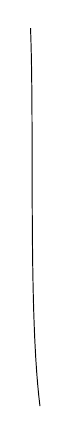
\begin{tikzpicture}[x=1cm,y=1cm]\draw[line width=.35pt] (0,0) .. controls (.05,-1.3) and (-.03,-3.6) .. (.12,-4.8);\end{tikzpicture}}}
\[
\begin{array}{@{}l@{\qquad}l@{}}
(1)&\displaystyle\boxed{\alpha_1\geq\alpha_2\mathord{.}\,\mathord{-}\,\mathord{-}\geq\alpha_n}\quad\text{and}\\
\text{\textcircled{2}}&\displaystyle\boxed{\boxed{\alpha_1+\mathord{-}\,\mathord{-}+\alpha_M\leq\beta_1+\mathord{-}+\beta_M\enspace\text{for }M=1,\mathord{-}\,\mathord{-}n.}}
\end{array}
\]

Let $\varphi(t_1,\mathord{-}\,\mathord{-}t_n)$ be a \uline{convex} and \uline{symmetric} numerical function on $R^n$. We assume that one of the following two conditions is satisfied: a) $\varphi$ is increasing \deleted{\unsure{(for}}\inserted{in each argument $t_i$} \deleted{the \unsure{natural order relation|restriction of a set} on $R^n$} b) $\sum_{i=1}^n\alpha_i=\sum_{i=1}^{n}\beta_i$.

{\reversemarginpar\margin{\begin{tikzpicture}[overlay,x=1cm,y=1cm]\draw[line width=.25pt] (.8,.2) .. controls (-.35,.4) and (-.35,-2.8) .. (.4,-3.1) .. controls (1.25,-3.5) and (2.1,-1.8) .. (1.9,-.1);\end{tikzpicture}\parbox[t]{1.85cm}{\unsure{function} where one \unsure{should} \unsure{allow} \unsure{H} \illegible{1} \deleted{\unsure{subset}} \unsure{an} open convex set.}}}

Under these conditions, we have
\[
\begin{array}{@{}l@{\qquad}l@{}}
(3)&\displaystyle\varphi(\alpha_1,\mathord{.}\,\mathord{-}\,\mathord{-},\alpha_n)\leq\varphi(\beta_1,\mathord{.}\,\mathord{-}\,\mathord{-}\beta_n)
\end{array}
\]

\deleted{Let us apply \unsure{at once} the following \unsure{corollary|lemma}, which \inserted{\unsure{alone us}} \illegible{1} \unsure{for the} \unsure{question} which \unsure{would erase} \illegible{1}. We immediately deduce from this the}

\deleted{\uline{Corollary 1}} \inserted{\textcircled{\uuline{2°}}} Let \inserted{$f(\rho_1,\mathord{-},\rho_n)$} be a \deleted{\uline{\unsure{continuous|numerical}}} \inserted{\uline{symmetric numerical}} function of $n$ \deleted{\unsure{positive}} arguments \inserted{$\rho_i>0$}, such that $f(e^{t_1},\mathord{-}\,\mathord{-},e^{t_n})$ is a \uline{convex} function of $(t_1,\mathord{-}\,\mathord{-}t_n)\in R^n$. Let $(\rho_1,\mathord{-}\rho_n)$ and $(\sigma_1,\mathord{-}\,\mathord{-},\sigma_n)$ be two \inserted{finite} positive sequences, such that \deleted{\unsure{(4bis)|(Hies.)}}

{\reversemarginpar\margin{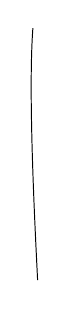
\begin{tikzpicture}[x=1cm,y=1cm]\draw[line width=.35pt] (0,0) .. controls (-.06,-.8) and (.02,-2.4) .. (.06,-3.2);\end{tikzpicture}}}
\[
\begin{array}{@{}l@{\qquad}l@{}}
\text{\textcircled{4}}&\displaystyle\boxed{\rho_1\geq\rho_2\mathord{-}\,\mathord{-}\geq\rho_n}\quad\text{and that }\deleted{\unsure{\sum\rho_i}}\\
\text{\textcircled{5}}&\displaystyle\boxed{\rho_1\mathord{.}\,\mathord{-}\rho_M\leq\sigma_1\mathord{.}\,\mathord{-}\sigma_M}\quad\text{for }\deleted{\text{all}}\ M=1,\mathord{-}n.
\end{array}
\]

We assume that one of the following two conditions is satisfied:

{\reversemarginpar\margin{It suffices that the set where $f$ is defined be a \unsure{suitable} \unsure{logarithmically} \unsure{convex} and symmetric subset.}}

a) $f$ is \inserted{defined and continuous for $\rho_i\geq0$, and} an increasing function \deleted{of the} \inserted{of} \deleted{\unsure{each of the} $\rho_i$}\inserted{each argument $\unsure{\sigma_i|\rho_i}$} b) $\rho_1\mathord{.}\,\mathord{-}\rho_n=\sigma_1\mathord{-}\,\mathord{-}\sigma_n\ne0$. Under these conditions, we have
\[
\begin{array}{@{}l@{\qquad}l@{}}
\deleted{\unsure{(4)}}\ (6)&\displaystyle f(\rho_1,\mathord{-}\,\mathord{-}\rho_n)\leq f(\sigma_1,\mathord{.}\,\mathord{-}\sigma_n)
\end{array}
\]

Indeed, if the $\rho_i,\sigma_i$ are $>0$, this statement is manifestly equivalent to the statement of the \deleted{lemma}\inserted{theorem}, on setting $\alpha_i=\log\rho_i$, $\beta_i=\log\sigma_i$. \inserted{This proves the \deleted{\unsure{corollary}}\inserted{(2°)} in particular in case b).}

{\reversemarginpar\margin{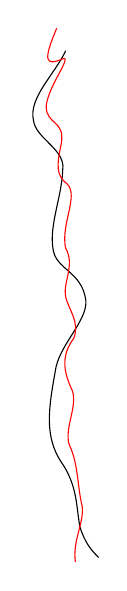
\begin{tikzpicture}[x=.0095cm,y=-.0095cm]
\draw[black] (65,37) .. controls (51,68) and (15,100) .. (22,130) .. controls (25,155) and (66,169) .. (61,197) .. controls (60,231) and (43,270) .. (48,301) .. controls (51,330) and (87,331) .. (92,371) .. controls (94,399) and (55,431) .. (51,466) .. controls (42,516) and (37,551) .. (58,585) .. controls (81,617) and (79,646) .. (84,673) .. controls (91,695) and (99,704) .. (109,714);
\draw[red] (53,7) .. controls (35,50) and (37,58) .. (61,48) .. controls (75,42) and (41,86) .. (39,111) .. controls (39,137) and (65,129) .. (59,162) .. controls (53,190) and (52,204) .. (67,215) .. controls (83,231) and (58,269) .. (65,301) .. controls (78,323) and (61,347) .. (65,366) .. controls (69,383) and (84,399) .. (76,421) .. controls (59,444) and (62,464) .. (72,487) .. controls (84,508) and (62,541) .. (70,564) .. controls (82,588) and (81,623) .. (87,645) .. controls (90,668) and (74,691) .. (78,720);
\end{tikzpicture}}}

\deleted{\unsure{We deduce from this}, since} \inserted{Let us show that} \inserted{in case a), every} \deleted{the set of} systems $(\rho_i),(\sigma_i)$ such that $\rho_i\geq0$, $\deleted{\unsure{\sigma_i\geq0|\rho_i>0}}$ \inserted{$\rho_1\geq\rho_2\mathord{-}\geq\rho_n\geq0$,} $\rho_1\mathord{.}\,\mathord{-}\mathord{.}\,\rho_M\leq\sigma_1\mathord{.}\,\mathord{-}\sigma_M$ for $M=1,\mathord{-}\,\mathord{-}n$, \deleted{(and \unsure{possibly|naturally} $\rho_1\mathord{.}\,\mathord{-}\rho_n=\sigma_1\mathord{-}\,\mathord{-}\sigma_n$)} \deleted{\unsure{is|and} the closure} \inserted{is a limit in $R^{2n}$} of \deleted{its subset consisting of systems such} \inserted{analogous systems} $(\rho'_i),(\sigma'_i)$ with $\rho'_i>0$, $\sigma'_i>0$ (whence will follow the \deleted{corollary}\inserted{(2°) in case a)} by extension by continuity). Indeed, if \deleted{\unsure{the $\rho_i$}} \inserted{$\sigma_i>0$ for all $i$,} one sees that by \deleted{\unsure{all cases}} increasing \inserted{by a sufficiently small amount} the $\rho_i$ which might be zero, \deleted{\unsure{are zero, and it suffices to approximate the systems}} one still satisfies the imposed conditions, \deleted{\unsure{and if} the systems $(\rho'_i),(\sigma'_i)$, with $\rho'_i=\sigma'_i=\frac1n$ for all $i$. \unsure{On the other hand|decreasing}} whence the conclusion \deleted{\unsure{desired|sought}}\inserted{in this case}.

{\reversemarginpar\margin{\unsure{{\color{red}?}}\kern-.3em\raisebox{-.7ex}{\unsure{{\color{black}?}}}}}

\deleted{If more generally, \unsure{in|therefore} \illegible{1} \unsure{one} \illegible{2} \unsure{which are} \illegible{1} first \illegible{1}}

{\reversemarginpar\margin{83}}
